\documentclass[11pt]{article}
\usepackage{graphicx}
\usepackage{hyperref}

\graphicspath{ {images/} }



\begin{document}
\title{Weekly Progress 1/25/2017}
\maketitle

\section{Introduction}
Created scripts to load datasets from UTIAS Multi-Robot Cooperative Localization and Mapping Datasets for simulations to verify our EFK works for a single robot localization. Later, we will expand to multirobots cooperative localization.

\section{Applied Data Sets}
There are 5 files needed for Robot1: \\

Landmark.dat, the locations of all 15 landmarks \\
\includegraphics[scale=0.4]{landmark}\\

\verb$Robot1_Groundtruth.dat$, the records of robot1's locations and orientations during the time\\
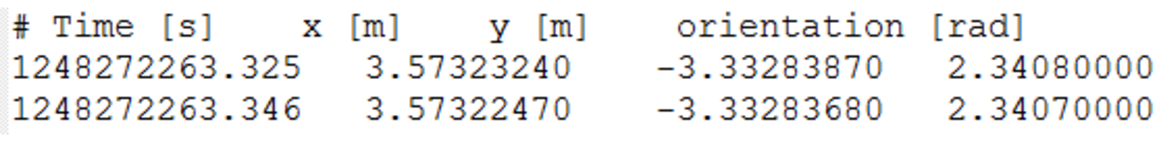
\includegraphics[scale=0.4]{R1_Groundtruth}\\

\verb$Robot1_Measurements.dat$, the records of robot1's measurment of the distances and angle of the objects robot detected\\
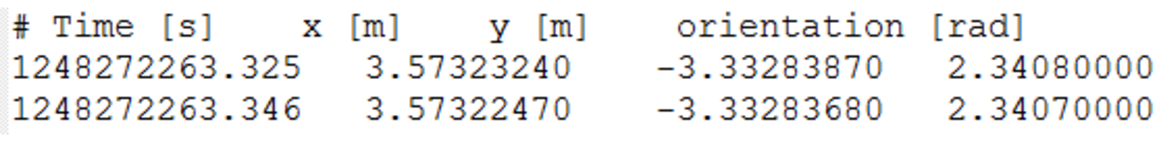
\includegraphics[scale=0.4]{R1_Groundtruth}\\

\verb$Robot1_Odometry.dat$, the records of robot1's speed and angular velocity during the time\\
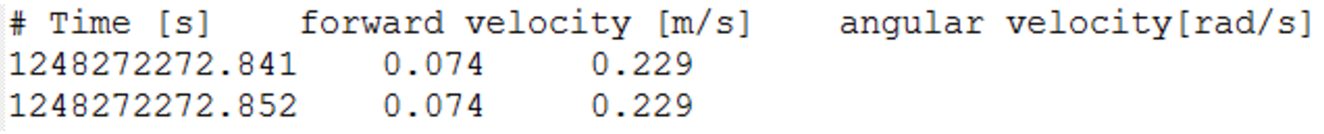
\includegraphics[scale=0.4]{R1_Odometry}\\


\verb$Barcode.dat$: translate between the barcodes the robot detect and the actual objects
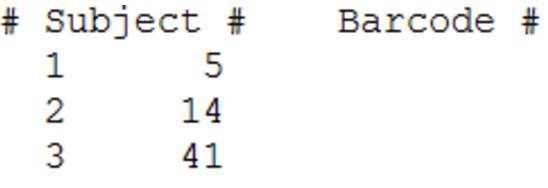
\includegraphics[scale=0.4]{Barcode}\\


\section{Mathematical Model}
There are two parts for EKF, state update and measurement update\\

State update:\\

\ $s_k = f (s_{k-1}, u) =  [s_{k-1}[1]+deltaT*i[1]*cos(s_{k-1}[3]); \\
         	  		s_{k-1}[2]+deltaT*i[1]*sin(s_{k-1}[3]); \\
         	  	 	s_{k-1}[3]+i[2]*deltaT]$ \\

Measurement Update: \\
\ $z_k = h(s,l) = [norm(l_k-s_k);  \\
             atan((l_k[2]-s_k[2])/(l_k[1]-s_k[1]))-s_k[3]];$ \\
             
Variables:
state of the robot(s): $s[1]$ is x-axis location, $s[2]$ is y-axis location and $s[3]$ is orientation

input(u): $[1]$ is velocity, $u[2]$is angular velocity

landmark(l): $l[1]$ is x-axis location, $l[2]$ is y-axis location 

measurement(z): $z[1]$ is the distance between the robot and the landmark, $z[2]$ is the bearing


$\frac{\partial Q}{\partial t} = \frac{\partial s}{\partial t}$





\section{Program Skeleton}
So far, there are 3 script files:\\
\url{git@git.uclalemur.com:billyskc/Localization_sim_py.git}\\

\verb$loc_sim.py$: this will give us the estimations of robot locations given odometry and measurement data. \\

\verb$comparison.py$: this will give us the groudtruth of the robot location within the time interval that match the localization performed by \verb$loc_sim.py$. \\

\verb$comparison_graph.m$: this will give us the graph of the robot's actual locations and estimate location in 2D. \\

\section{Progress and Results}
Past few week, we create a single matlab script to do the simulation. Because of the sizes of all these data files, it took a long time (1-2 mins) for each run, which makes it difficult to debug. More importantly, Octave graphic toolkit doesn't work well on my laptop. My laptop kept crashing even with gnuplot.  

We decide to switch to python and only use matlab for graphing purpose. Now, these scripts are compiled much faster and crashing issue is solved as well. 

Here is the plot for 1000 time step after Robot1 start to move: \\
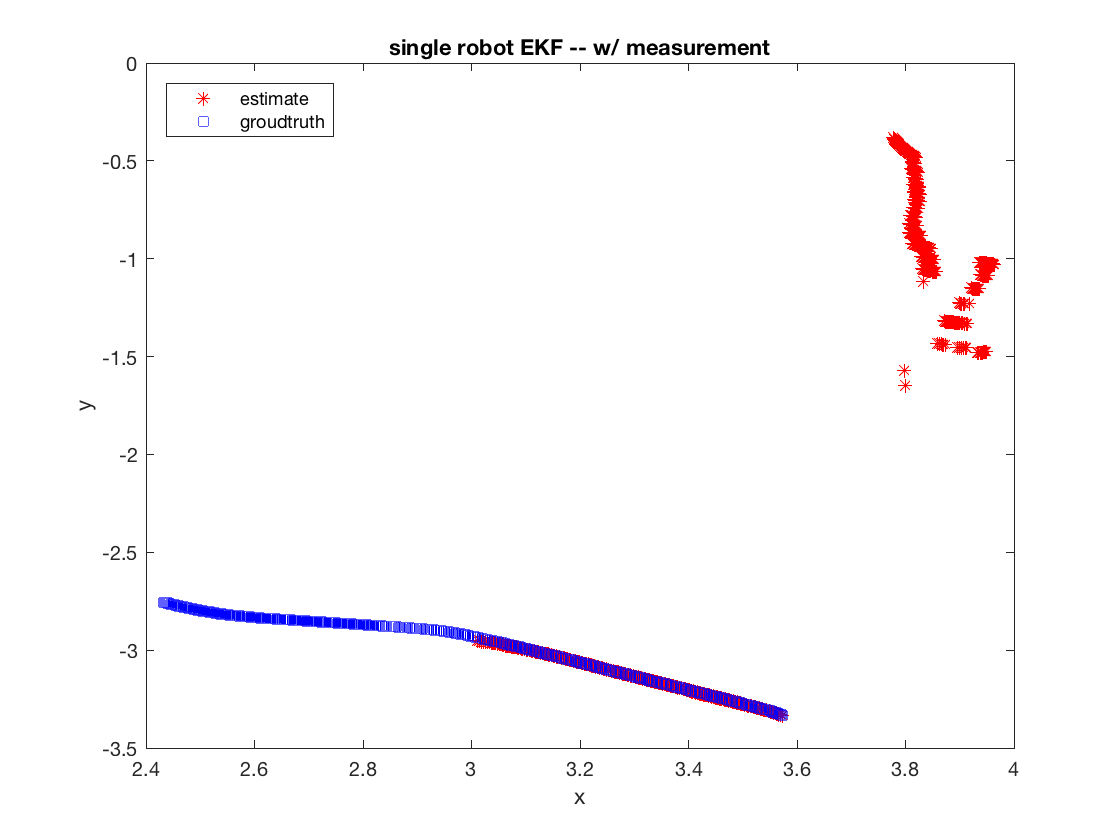
\includegraphics[scale = 0.3]{Single_EKF_incorrect}\\

When time around t= 1248272284.671, estimations no longer stay near groudtruth. There are several measurements have been taken already.


\section{Next Week Plan}
Keep debugging 



\end{document}